\begin{figure}[H]
  \centering
  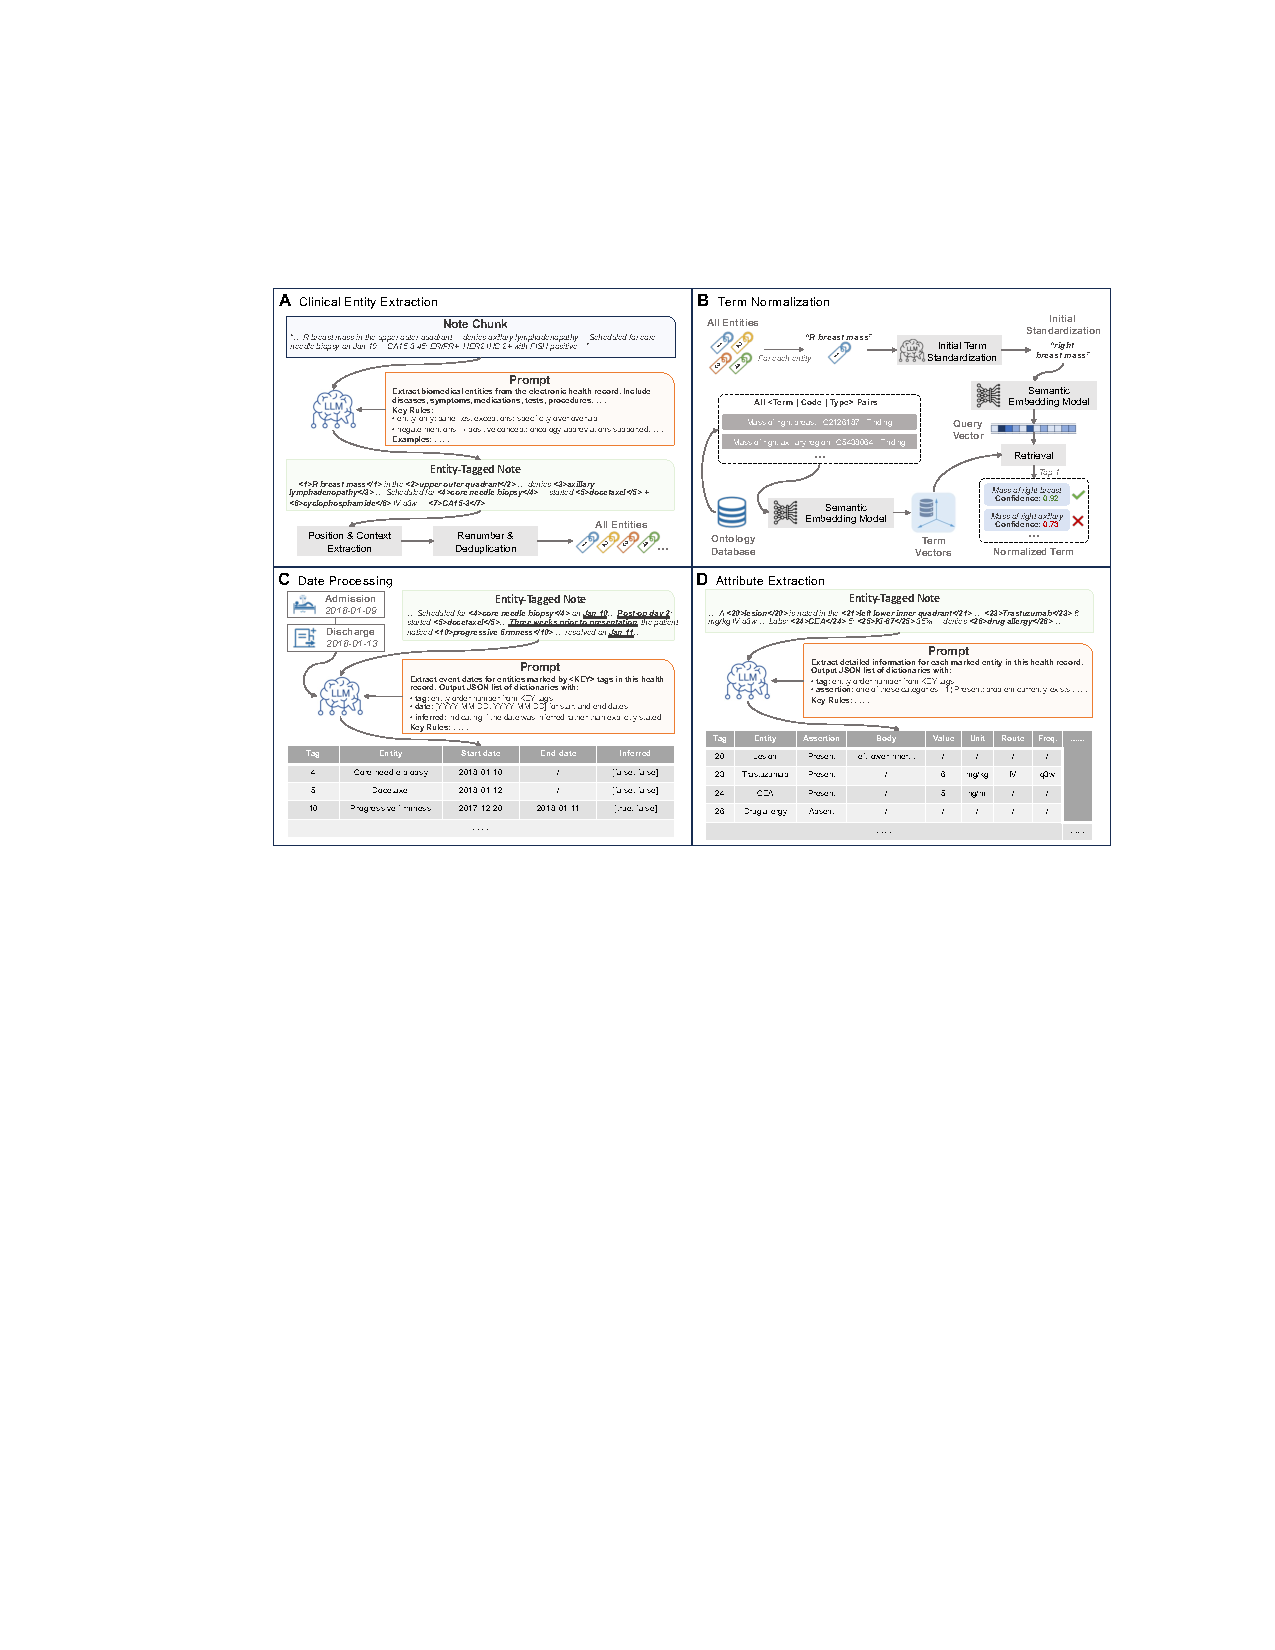
\includegraphics[width=\linewidth,height=0.9\textheight,keepaspectratio]{figures/figure2.pdf}\vspace{-8mm}
  \caption{\textbf{CLINES LLM-based module workflow.} (A) Within each note chunk, the LLM tags clinical entities; post-processing yields an entity list with source offsets and a surrounding context window. (B) The LLM performs preliminary normalization, after which an embedding-based retriever queries the ontology database to return the nearest term, concept code, and semantic type. (C) Explicit dates/times are extracted from local context; when documentation is vague, admission/discharge metadata are used to resolve relative or fuzzy expressions to the most plausible calendar dates. (D) Context is used to capture modifiers (e.g., for medications: dose, unit, frequency, route; for tests: numeric values and units; for diseases: activity status), and to infer latent modifiers implied by panel tests (e.g., default units). All machine-inferred fields are flagged as ``inferred'' to facilitate audit and downstream use.}
  \label{fig:clines-workflow}
\end{figure}
